\documentclass[a4paper,10pt]{article}
\usepackage[utf8]{inputenc}
\usepackage[margin=1.5cm, bottom=2cm]{geometry}
\usepackage{fancyhdr}
\usepackage{enumitem}
\usepackage{xcolor}
\usepackage[most]{tcolorbox}
\newtcolorbox{osservazioni}{
  colback=gray!8,    % sfondo grigio chiaro
  colframe=white,      % nessun bordo
  arc=2mm,            % angoli smussati
  boxrule=0pt,        % spessore bordo 0
  fontupper=\footnotesize,
  left=2mm, right=2mm, top=2mm, bottom=2mm,
  before skip=7pt,   % niente spazio prima
  after skip=15pt     % niente spazio dopo
}
\pagestyle{fancy}
\usepackage{tikz}
\usetikzlibrary{automata, positioning}
\pagestyle{fancy}


%%%%%%%%%%%%%%%%%%%
\newcommand{\EsercitazioneNum}{01}
\newcommand{\Data}{25/09/2025}
%%%%%%%%%%%%%%%%%%%

% Numero di pagina in basso al centro
\fancyhf{}
\fancyfoot[C] \thepage
\renewcommand{\footrulewidth}{0pt} % niente linea in basso
\renewcommand{\headrulewidth}{0pt} % niente linea in alto

\begin{document}
\footnotesize  % font generale più piccolo

\noindent
\small \textbf{Computabilità, Complessità e Logica - a.a. 2025/26} \hfill \textbf{Esercitazione \EsercitazioneNum} \\[0.2cm]
\scriptsize Matteo Liotta, \texttt{matteo.liotta@studenti.units.it} \hfill \Data \\[0.2cm]

\noindent\makebox[\linewidth]{\rule{\linewidth}{0.4pt}} \\[1cm]


\noindent\Large \textbf{Esercitazione 01}: \textit{Macchine a stati finiti e Linguaggi Regolari}\\[0.4cm]
{\normalsize
\begin{itemize}[label=, leftmargin=0pt]

    \item \textbf{Esercizio 1. (*)}\\
    Si consideri il seguente automa regolare su $\Sigma = \{a,b,c \}$:
    {
    \small
    \begin{center}
    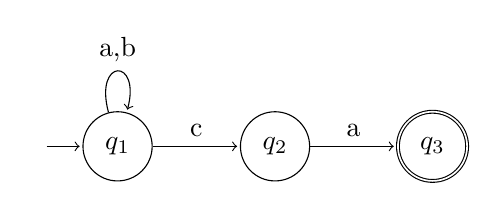
\begin{tikzpicture}[shorten >=1pt, node distance=2cm, on grid, auto]
        \node[state, initial, initial text=] (q1)   {$q_1$};
        \node[state] (q2) [right=of q1] {$q_2$};
        \node[state, accepting] (q3) [right=of q2] {$q_3$};
        
        \path[->]
        (q1) edge [loop above] node {a,b} (q1)
             edge node {c} (q2)
        (q2) edge node {a} (q3);
        
         
    \end{tikzpicture}
    \end{center}
    }
    Si identifichi il linguaggio riconosciuto dall'automa.
 
    \item \textbf{Esercizio 2. (*)}\\ Sia $L$ linguaggio regolare su $\Sigma=\{a,b\}$, tale per cui 
    {\\ \begin{center}
        $L = \{ w\in \Sigma^* \mid w \text{\ ha\ un\ numero\ pari\ di\ } a \}$\\
    \end{center}}
    Si rappresenti l'automa regolare che riconosce tale linguaggio.


    
    \item \textbf{Esercizio 3. (*)}\\ Sia $L$ linguaggio regolare su $\Sigma=\{a,b\}$, tale per cui 
    {\\ \begin{center}
        $L = \{ w \in \Sigma^* \mid w = (ab)^n, n>0 \}$
    \end{center}} 
    Si rappresenti l'automa regolare che riconosce tale linguaggio.



    
 
    
    \item \textbf{Esercizio 4. (**)}\\ Sia $L$ linguaggio regolare su $\Sigma=\{a,b\}$, tale per cui 
    {\\ \begin{center}
        $L = \{ w \in \Sigma^*\mid w \text{\ ha\ un\ numero\ pari\ di\ "a"} e\text{\ un\ numero\ dispari\ di\ "b"}\}$
    \end{center}} 
    Si rappresenti l'automa regolare che riconosce tale linguaggio.



    \item \textbf{Esercizio 5. (***)}\\ Sia $L$ linguaggio su $\Sigma=\{a,b\}$, tale per cui 
    {\\ \begin{center}
        $L = \{ w \in \Sigma^* \mid \#a = \#b\ in\ w\}$
    \end{center}} 
    Si rappresenti, se possibile, l'automa regolare che riconosce tale linguaggio.

    \item \textbf{Esercizio 6. (**)}\\
    Si considerino i seguenti automi regolari su $\Sigma = \{0,1\}$:
    {
    \small
    \begin{center}
    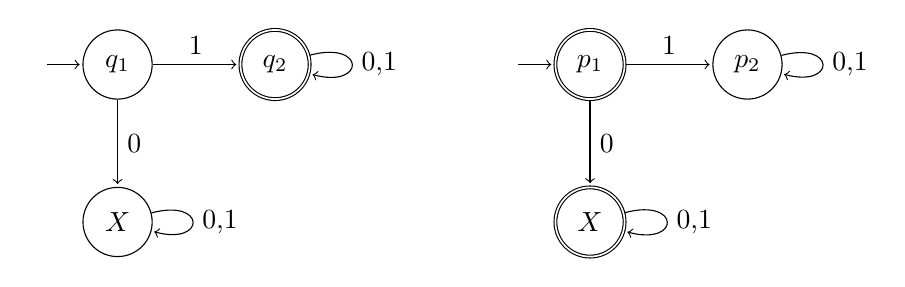
\begin{tikzpicture}[shorten >=1pt, node distance=2cm, on grid, auto]
        
        \node[state, initial, initial text=] (q1) {$q_1$};
        \node[state, right=of q1, accepting] (q2) {$q_2$};
        \node[state, below=of q1] (X1) {$X$};

        \node[state, right=4cm of q2, initial, accepting, initial text=] (p1) {$p_1$};
        \node[state, right=of p1] (p2) {$p_2$};
        \node[state, below=of p1, accepting] (X2) {$X$};
        
        \path[->]
        (q1) edge node {1} (q2)
             edge node {0} (X1)
        (q2) edge [loop right] node {0,1} ()
        (X1) edge [loop right] node {0,1} ()
        
        (p1) edge node {1} (p2)
             edge node {0} (X2)
        (p2) edge [loop right] node {0,1} ()
        (X2) edge [loop right] node {0,1} ();

    \end{tikzpicture}
    \end{center}
    }
    Si identifichino i linguaggi riconosciuti. Si può osservare qualche relazione tra loro?

\vfill
\noindent\makebox[\linewidth]{\rule{\linewidth}{0.4pt}}

    \newpage
    {\noindent
    \small \textbf{Computabilità, Complessità e Logica - a.a. 2025/26} \hfill \textbf{Esercitazione \EsercitazioneNum} \\[0.2cm]
    \scriptsize Matteo Liotta, \texttt{matteo.liotta@studenti.units.it} \hfill \Data \\[0.2cm]
    \noindent\makebox[\linewidth]{\rule{\linewidth}{0.4pt}} \\[0.3cm]}



    %\item \textbf{Esercizio 7. (***)}\\ Sia $L$ un linguaggio regolare su $\Sigma$. Si dimostri la regolarità del seguente %linguaggio su $\Sigma$:
    %{\begin{center}
    %    $L_1 = \{w\in L\mid \forall \ x,y\in \Sigma^*, \ x\neq w \Rightarrow  x\notin L\}$
    %\end{center}} 

    \item \textbf{Esercizio 7. (***)}\\ Sia $L$ un linguaggio regolare su $\Sigma$. Si dimostri la regolarità del seguente linguaggio su $\Sigma$:
    {\begin{center}
        $L_{2} = \{x\in \Sigma^*\mid \exists y\in\Sigma^*\ \text{con}\ \ xy\in L \}$
    \end{center}} 
    Si definisca inoltre la relazione che sussiste tra $L$ ed $L_2$, tra le seguenti: $L\subset L_2$, $L_2 \subset L$, $L\equiv L_2$.
    
    

\end{itemize}
}
\vfill
\noindent\makebox[\linewidth]{\rule{\linewidth}{0.1pt}}
\end{document}
